 \documentclass[12pt, titlepage]{article}

\usepackage{fullpage}
\usepackage[round]{natbib}
\usepackage{multirow}
\usepackage{booktabs}
\usepackage{tabularx}
\usepackage{graphicx}
\usepackage{float}
\usepackage{hyperref}
\hypersetup{
    colorlinks,
    citecolor=blue,
    filecolor=black,
    linkcolor=red,
    urlcolor=blue
}

%% Comments

\usepackage{color}

\newif\ifcomments\commentstrue %displays comments
%\newif\ifcomments\commentsfalse %so that comments do not display

\ifcomments
\newcommand{\authornote}[3]{\textcolor{#1}{[#3 ---#2]}}
\newcommand{\todo}[1]{\textcolor{red}{[TODO: #1]}}
\else
\newcommand{\authornote}[3]{}
\newcommand{\todo}[1]{}
\fi

\newcommand{\wss}[1]{\authornote{blue}{SS}{#1}} 
\newcommand{\plt}[1]{\authornote{magenta}{TPLT}{#1}} %For explanation of the template
\newcommand{\an}[1]{\authornote{cyan}{Author}{#1}}
%% Common Parts

\newcommand{\progname}{ProgName} % PUT YOUR PROGRAM NAME HERE
\newcommand{\authname}{Team \#, Team Name
\\ Student 1 name and macid
\\ Student 2 name and macid
\\ Student 3 name and macid
\\ Student 4 name and macid} % AUTHOR NAMES                  

\usepackage{hyperref}
    \hypersetup{colorlinks=true, linkcolor=blue, citecolor=blue, filecolor=blue,
                urlcolor=blue, unicode=false}
    \urlstyle{same}
                                


\newcounter{acnum}
\newcommand{\actheacnum}{AC\theacnum}
\newcommand{\acref}[1]{AC\ref{#1}}

\newcounter{ucnum}
\newcommand{\uctheucnum}{UC\theucnum}
\newcommand{\uref}[1]{UC\ref{#1}}

\newcounter{mnum}
\newcommand{\mthemnum}{M\themnum}
\newcommand{\mref}[1]{M\ref{#1}}

%self defined command
\newcommand{\UUI}{Unity(UI From Unity Engine).}

\begin{document}

\title{Module Guide for \progname{}} 
\author{\authname}
\date{\today}

\maketitle

\pagenumbering{roman}

\section{Revision History}

\begin{tabularx}{\textwidth}{p{3cm}p{2cm}X}
\toprule {\bf Date} & {\bf Version} & {\bf Notes}\\
\midrule
Jan 14 & 1.0 & First Version\\
\hline
April 2 & 2.0 & Final Draft \\
\bottomrule
\end{tabularx}

\newpage

\section{Reference Material}

This section records information for easy reference.

\subsection{Abbreviations and Acronyms}

\renewcommand{\arraystretch}{1.2}
\begin{tabular}{l l} 
  \toprule		
  \textbf{symbol} & \textbf{description}\\
  \midrule 
  AC & Anticipated Change\\
  DAG & Directed Acyclic Graph \\
  M & Module \\
  MG & Module Guide \\
  OS & Operating System \\
  R & Requirement\\
  FR & Functional Requirement\\
  NFR & Non-Functional Requirement\\
  SC & Scientific Computing \\
  SRS & Software Requirements Specification\\
  \progname & Explanation of program name\\
  UC & Unlikely Change \\
  MVC & Model, Viewer, Controller\\
  GUI & Graphical User Interface\\
  LAI & Leaf Area Index\\
  DBH & Diameter at breast height\\
  \bottomrule
\end{tabular}\\

\newpage

\tableofcontents

\listoftables

\listoffigures

\newpage

\pagenumbering{arabic}

\section{Introduction}

Decomposing a system into modules is a commonly accepted approach to developing
software.  A module is a work assignment for a programmer or programming
team~\citep{ParnasEtAl1984}.  We advocate a decomposition
based on the principle of information hiding~\citep{Parnas1972a}.  This
principle supports design for change, because the ``secrets'' that each module
hides represent likely future changes.  Design for change is valuable in SC,
where modifications are frequent, especially during initial development as the
solution space is explored.  

Our design follows the rules layed out by \citet{ParnasEtAl1984}, as follows:
\begin{itemize}
\item System details that are likely to change independently should be the
  secrets of separate modules.
\item Each data structure is implemented in only one module.
\item Any other program that requires information stored in a module's data
  structures must obtain it by calling access programs belonging to that module.
\end{itemize}

\noindent After completing the first stage of the design, the Software Requirements
Specification (SRS), the Module Guide (MG) is developed~\citep{ParnasEtAl1984}. The MG
specifies the modular structure of the system and is intended to allow both
designers and maintainers to easily identify the parts of the software.  The
potential readers of this document are as follows:

\begin{itemize}
\item New project members: This document can be a guide for a new project member
  to easily understand the overall structure and quickly find the
  relevant modules they are searching for.
\item Maintainers: The hierarchical structure of the module guide improves the
  maintainers' understanding when they need to make changes to the system. It is
  important for a maintainer to update the relevant sections of the document
  after changes have been made.
\item Designers: Once the module guide has been written, it can be used to
  check for consistency, feasibility, and flexibility. Designers can verify the
  system in various ways, such as consistency among modules, feasibility of the
  decomposition, and flexibility of the design.
\end{itemize}

\noindent The rest of the document is organized as follows. Section
\ref{SecChange} lists the anticipated and unlikely changes of the software
requirements. Section \ref{SecMH} summarizes the module decomposition that
was constructed according to the likely changes. Section \ref{SecConnection}
specifies the connections between the software requirements and the
modules. Section \ref{SecMD} gives a detailed description of the
modules. Section \ref{SecTM} includes two traceability matrices. One checks
the completeness of the design against the requirements provided in the SRS. The
other shows the relation between anticipated changes and the modules. Section
\ref{SecUse} describes the use relation between modules.\\

\noindent \textcolor{red}{Notes: We use MVC as our software architecture, therefore, we 
decomposed our modules according to models, viewers, and controllers.}

\section{Anticipated and Unlikely Changes} \label{SecChange}

This section lists possible changes to the system. According to the likeliness
of the change, the possible changes are classified into two
categories. Anticipated changes are listed in Section \ref{SecAchange}, and
unlikely changes are listed in Section \ref{SecUchange}.

\subsection{Anticipated Changes} \label{SecAchange}

Anticipated changes are the source of the information that is to be hidden
inside the modules. Ideally, changing one of the anticipated changes will only
require changing the one module that hides the associated decision. The approach
adapted here is called design for
change.

\begin{description}
\item[\refstepcounter{acnum} \actheacnum \label{acMainUI}:] The UI appearance of the main page
 will be continuously upgraded.
 
\item[\refstepcounter{acnum} \actheacnum \label{acDataDisplay}:] The way of displaying 
environmental data and tree parameters may change.

\item[\refstepcounter{acnum} \actheacnum \label{acDataValue}:] The values of
environmental data and tree parameters may change.

\item[\refstepcounter{acnum} \actheacnum \label{acTreeParam}:] Tree parameters of different
trees may change. For example, the stakeholders may add different tree parameters for 
different types of trees in the future.

\item[\refstepcounter{acnum} \actheacnum \label{acEnvData}:] The stakeholders may add more
environmental data in the future.

\end{description}

\subsection{Unlikely Changes} \label{SecUchange}

The module design should be as general as possible. However, a general system is
more complex. Sometimes this complexity is not necessary. Fixing some design
decisions at the system architecture stage can simplify the software design. If
these decision should later need to be changed, then many parts of the design
will potentially need to be modified. Hence, it is not intended that these
decisions will be changed.

\begin{description}
\item[\refstepcounter{ucnum} \uctheucnum \label{ucIO}:]  IO devices(keyboard \& mouse). 
\item[\refstepcounter{ucnum} \uctheucnum \label{ucOS}:] The system will always run on 
macOS and Windows. 
\item[\refstepcounter{ucnum} \uctheucnum \label{ucModel}:] The 3D model of the virtual forest.
\item[\refstepcounter{ucnum} \uctheucnum \label{ucMove}:] The way of viewing forest models.
\end{description}


\newpage

\section{Module Hierarchy} \label{SecMH}

This section provides an overview of the module design. Modules are summarized
in a hierarchy decomposed by secrets in Table \ref{TblModels}, \ref{TblViewers1}, \ref{TblViewers2},
and \ref{TblControllers}. The modules listed
below, which are leaves in the hierarchy tree, are the modules that will
actually be implemented.

\begin{table}[H]
\caption{Module Hierarchy(Models)}
\label{TblModels}

\centering
\begin{tabular}{p{0.3\textwidth} p{0.6\textwidth}}
\toprule
\textbf{Level 1} & \textbf{Level 2}\\
\midrule

\multirow{14}{0.3\textwidth}{Model Modules}
& \refstepcounter{mnum} \mthemnum \label{Model1}: ForestTrees \\
& \refstepcounter{mnum} \mthemnum \label{Model2}: ForestSky  \\
& \refstepcounter{mnum} \mthemnum \label{Model3}: ForestTerrain \\
& \refstepcounter{mnum} \mthemnum \label{Model4}: RedPine  \\
& \refstepcounter{mnum} \mthemnum \label{Model5}: Oak   \\
& \refstepcounter{mnum} \mthemnum \label{Model6}: Beech  \\
& \refstepcounter{mnum} \mthemnum \label{Model7}: Birch  \\ 
& \refstepcounter{mnum} \mthemnum \label{Model8}: WhitePine  \\
& \refstepcounter{mnum} \mthemnum \label{Model9}: RedMaple \\
& \refstepcounter{mnum} \mthemnum \label{Model10}: RedOak  \\
& \refstepcounter{mnum} \mthemnum \label{Model11}: EnvData  \\
& \refstepcounter{mnum} \mthemnum \label{Model12}: PlotData  \\
& \refstepcounter{mnum} \mthemnum \label{Model13}: FirstPersonPlayer  \\
& \refstepcounter{mnum} \mthemnum \label{Model14}: JsonFile  \\
\bottomrule

\end{tabular}

\end{table}


\newpage

\begin{table}[H]
\caption{Module Hierarchy(First Viewers Table)}
\label{TblViewers1}

\centering
\begin{tabular}{p{0.3\textwidth} p{0.6\textwidth}}
\toprule
\textbf{Level 1} & \textbf{Level 2}\\
\midrule

\multirow{13}{0.3\textwidth}{Viewer Modules}
& \refstepcounter{mnum} \mthemnum \label{Viwer1}: MainPageDisplay \\
& \refstepcounter{mnum} \mthemnum \label{Viwer2}: StartButton \\
& \refstepcounter{mnum} \mthemnum \label{Viwer3}: InstructionButton \\
& \refstepcounter{mnum} \mthemnum \label{Viwer4}: ContactUsButton \\
& \refstepcounter{mnum} \mthemnum \label{Viwer5}: QuitButton \\
& \refstepcounter{mnum} \mthemnum \label{Viwer6}: InstructionInfoDisplay \\
& \refstepcounter{mnum} \mthemnum \label{Viwer7}: ContactUsInfoDisplay \\ 
& \refstepcounter{mnum} \mthemnum \label{Viwer8}: BackButton \\
& \refstepcounter{mnum} \mthemnum \label{Viwer9}: UpdateDataDisplay \\
& \refstepcounter{mnum} \mthemnum \label{Viwer10}: EnvDataSelectionButton \\
& \refstepcounter{mnum} \mthemnum \label{Viwer11}: DataTypeSelectionButtons \\
& \refstepcounter{mnum} \mthemnum \label{Viwer12}: NewDataInputBox \\
& \refstepcounter{mnum} \mthemnum \label{Viwer13}: SaveButton \\
\bottomrule
\end{tabular}
\end{table}

\newpage

\begin{table}[H]
\caption{Module Hierarchy(Second Viewers Table)}
\label{TblViewers2}

\centering
\begin{tabular}{p{0.3\textwidth} p{0.6\textwidth}}
\toprule
\textbf{Level 1} & \textbf{Level 2}\\
\midrule

\multirow{10}{0.3\textwidth}{Viewer Modules}
& \refstepcounter{mnum} \mthemnum \label{Viwer14}: CurrentDataDisplay \\
& \refstepcounter{mnum} \mthemnum \label{Viwer15}: PlotSelectionDropDown \\
& \refstepcounter{mnum} \mthemnum \label{Viwer16}: TreeTypeSelectionDropDown \\
& \refstepcounter{mnum} \mthemnum \label{Viwer17}: UpdateDataButton \\
& \refstepcounter{mnum} \mthemnum \label{Viwer18}: ForestDisplay \\
& \refstepcounter{mnum} \mthemnum \label{Viwer19}: ShowEnvDataButton \\
& \refstepcounter{mnum} \mthemnum \label{Viwer20}: ShowTreeParamButton \\
& \refstepcounter{mnum} \mthemnum \label{Viwer21}: EnvDataDisplay \\
& \refstepcounter{mnum} \mthemnum \label{Viwer22}: TreeParamDisplay \\
& \refstepcounter{mnum} \mthemnum \label{Viwer23}: PauseIndicatorDisplay \\
\bottomrule
\end{tabular}
\end{table}

\newpage

\begin{table}[H]
\caption{Module Hierarchy(Controllers)}
\label{TblControllers}

\centering
\begin{tabular}{p{0.3\textwidth} p{0.6\textwidth}}
\toprule
\textbf{Level 1} & \textbf{Level 2}\\
\midrule

\multirow{18}{0.3\textwidth}{Controller Modules}
& \refstepcounter{mnum} \mthemnum \label{Controller1}: JsonFileReader \\
& \refstepcounter{mnum} \mthemnum \label{Controller2}: JsonFileWriter  \\
& \refstepcounter{mnum} \mthemnum \label{Controller3}: PauseManager  \\
& \refstepcounter{mnum} \mthemnum \label{Controller4}: PlayerMovement  \\
& \refstepcounter{mnum} \mthemnum \label{Controller5}: NewDataInputBoxController\\
& \refstepcounter{mnum} \mthemnum \label{Controller6}: StartButtonController  \\
& \refstepcounter{mnum} \mthemnum \label{Controller7}: InstructionButtonController \\
& \refstepcounter{mnum} \mthemnum \label{Controller8}: UpdateDataButtonController\\
& \refstepcounter{mnum} \mthemnum \label{Controller9}: ContactUsButtonController \\
& \refstepcounter{mnum} \mthemnum \label{Controller10}: QuitButtonController  \\
& \refstepcounter{mnum} \mthemnum \label{Controller11}: BackButtonController \\
& \refstepcounter{mnum} \mthemnum \label{Controller12}: PlotSelectionDropDownController \\
& \refstepcounter{mnum} \mthemnum \label{Controller13}: TreeTypeSelectionDropDownController \\
& \refstepcounter{mnum} \mthemnum \label{Controller14}: ShowEnvDataButtonController \\
& \refstepcounter{mnum} \mthemnum \label{Controller15}: ShowTreeParamButtonController \\
& \refstepcounter{mnum} \mthemnum \label{Controller16}: EnvDataSelectionButtonController\\
& \refstepcounter{mnum} \mthemnum \label{Controller17}: DataTypeSelectionButtonsController \\
& \refstepcounter{mnum} \mthemnum \label{Controller18}: SaveButtonController \\
\bottomrule

\end{tabular}

\end{table}

\newpage

\section{Connection Between Requirements and Design} \label{SecConnection}

The design of the system is intended to satisfy the requirements developed in
the SRS(click \href{https://github.com/wuj187/DigitalTwinCAS/blob/main/docs/DocRevision/SRSRevision/SRSRevision.pdf}{here} for revised SRS). In this stage, the system is decomposed into modules. The connection
between functional requirements and modules is listed in Table~\ref{TbFRM}. 
The connection
between non-functional requirements and modules is listed in Table~\ref{TbNFRM1} and \ref{TbNFRM2}.

\section{Module Decomposition} \label{SecMD}

Modules are decomposed according to the principle of ``information hiding''
proposed by \citet{ParnasEtAl1984}. The \emph{Secrets} field in a module
decomposition is a brief statement of the design decision hidden by the
module. The \emph{Services} field specifies \emph{what} the module will do
without documenting \emph{how} to do it. For each module, a suggestion for the
implementing software is given under the \emph{Implemented By} title. 

\begin{itemize}
\item If the
entry is \emph{OS}, this means that the module is provided by the operating
system or by standard programming language libraries. 

\item If the entry is \emph{Unity}, this means that the module is provide by libraries from
Unity Engine.

\item \emph{\progname{}} means the
module will be implemented by the \progname{} software
\end{itemize}

\subsection{Model Modules}

\subsubsection{ForestTrees Module (\mref{Model1})}
\begin{description}
\item[Secrets:] How the tree models are displayed.
\item[Services:] Provide virtual trees for the virtual forest.
\item[Implemented By:] \progname{} and Unity(Unity libraries are used to help build tree
models)
\end{description}

\subsubsection{ForestSky Module (\mref{Model2})}
\begin{description}
\item[Secrets:] How the skybox and light are displayed.
\item[Services:] Provide virtual sky for the virtual forest.
\item[Implemented By:] \progname{} Unity(Unity libraries are used to help build forest sky)
\end{description}

\subsubsection{ForestTerrain Module (\mref{Model3})}
\begin{description}
\item[Secrets:] How the ground textures are displayed.
\item[Services:] Provide virtual terrain for the virtual forest.
\item[Implemented By:] \progname{} Unity(Unity libraries are used to help build forest 
terrain)
\end{description}

\subsubsection{RedPine Module (\mref{Model4})}
\begin{description}
\item[Secrets:] Attributes of red pine trees and associated methods about these attributes.
\item[Services:] Allow developers to define objects of red pine trees. From the objects, developers can store,
read, or reset attributes about the red pine trees.
\item[Implemented By:] \progname{}
\end{description}


\subsubsection{Oak Module (\mref{Model5})}
\begin{description}
\item[Secrets:] Attributes of oak trees and associated methods about these attributes.
\item[Services:] Allow developers to define objects of oak trees. From the objects, developers can store,
read, or reset attributes about the oak trees.
\item[Implemented By:] \progname{}
\end{description}

\newcommand\tn{beech }
\newcommand\TN{Beech }
\subsubsection{\TN Module (\mref{Model6})}
\begin{description}
\item[Secrets:] Attributes of \tn trees and associated methods about these attributes.
\item[Services:] Allow developers to define objects of \tn trees. From the objects, developers can store,
read, or reset attributes about the \tn trees.
\item[Implemented By:] \progname{}
\end{description}

\renewcommand\tn{birch }
\renewcommand\TN{Birch }
\subsubsection{\TN Module (\mref{Model7})}
\begin{description}
\item[Secrets:] Attributes of \tn trees and associated methods about these attributes.
\item[Services:] Allow developers to define objects of \tn trees. From the objects, developers can store,
read, or reset attributes about the \tn trees.
\item[Implemented By:] \progname{}
\end{description}

\renewcommand\tn{white pine }
\renewcommand\TN{WhitePine }
\subsubsection{\TN Module (\mref{Model8})}
\begin{description}
\item[Secrets:] Attributes of \tn trees and associated methods about these attributes.
\item[Services:] Allow developers to define objects of \tn trees. From the objects, developers can store,
read, or reset attributes about the \tn trees.
\item[Implemented By:] \progname{}
\end{description}

\renewcommand\tn{red maple }
\renewcommand\TN{RedMaple }
\subsubsection{\TN Module (\mref{Model9})}
\begin{description}
\item[Secrets:] Attributes of \tn trees and associated methods about these attributes.
\item[Services:] Allow developers to define objects of \tn trees. From the objects, developers can store,
read, or reset attributes about the \tn trees.
\item[Implemented By:] \progname{}
\end{description}

\renewcommand\tn{red oak }
\renewcommand\TN{RedOak }
\subsubsection{\TN Module (\mref{Model10})}
\begin{description}
\item[Secrets:] Attributes of \tn trees and associated methods about these attributes.
\item[Services:] Allow developers to define objects of \tn trees. From the objects, developers can store,
read, or reset attributes about the \tn trees.
\item[Implemented By:] \progname{}
\end{description}

\subsubsection{EnvData Module (\mref{Model11})}
\begin{description}
\item[Secrets:] Attributes of plot environment and associated methods about these attributes.
\item[Services:] Allow developers to define objects of plot environment. From the objects,
 developers can store, read, or reset attributes about the plot environment.
\item[Implemented By:] \progname{}
\end{description}

\subsubsection{PlotData Module (\mref{Model12})}
\begin{description}
\item[Secrets:] Attributes of a plot and associated methods about these attributes. Attributes
for a plot include plot environment attributes and different types of trees' attributes 
within this plot.
\item[Services:] Allow developers to define objects of a plot. From the objects,
 developers can store, read, or reset attributes about the plot.
\item[Implemented By:] \progname{}
\end{description}

\subsubsection{FirstPersonPlayer Module (\mref{Model13})}
\begin{description}
\item[Secrets:] The algorithms to control first person view movement in the virtual forest.
\item[Services:] Allow users to move and navigate through the forest to browse trees, terrain,
sky. etc.
\item[Implemented By:] \progname{}
\end{description}

\subsubsection{JsonFile Module (\mref{Model14})}
\begin{description}
\item[Secrets:] Data structure to for storing environment data and tree parameters.
\item[Services:] Json files are used to store data for our system. There are modules to 
read/write data from/to json files in order to display data on the screen and update data.
\item[Implemented By:] \progname{}
\end{description}

\subsection{Viewer Modules}

\subsubsection{MainPageDisplay Module (\mref{Viwer1})}
\begin{description}
\item[Secrets:] A GUI which contains background image and different buttons.
\item[Services:] Provide users some options at the beginning of the software. Options include
starting browsing virtual forest, checking instructions, checking team members' contact
information, quitting the software.
\item[Implemented By:] \progname{} and Unity(UI From Unity Engine).
\end{description}


\newcommand\bt{\textbf{Start }}
\subsubsection{StartButton Module (\mref{Viwer2})}
\begin{description}
\item[Secrets:] A GUI of the \bt button.
\item[Services:] Provide a button GUI for users to start browsing virtual forest after 
clicking it.
\item[Implemented By:] Unity(UI From Unity Engine).
\end{description}

\renewcommand\bt{\textbf{Instruction }}
\subsubsection{InstructionButton Module (\mref{Viwer3})}
\begin{description}
\item[Secrets:] A GUI of the \bt button.
\item[Services:] Provide a button GUI for users to check software instructions after 
clicking it.
\item[Implemented By:] Unity(UI From Unity Engine).
\end{description}

\renewcommand\bt{\textbf{Contact Us }}
\subsubsection{ContactUsButton Module (\mref{Viwer4})}
\begin{description}
\item[Secrets:] A GUI of the \bt button.
\item[Services:] Provide a button GUI for users to check team members' information after 
clicking it.
\item[Implemented By:] Unity(UI From Unity Engine).
\end{description}

\renewcommand\bt{\textbf{Quit }}
\subsubsection{QuitButton Module (\mref{Viwer5})}
\begin{description}
\item[Secrets:] A GUI of the \bt button.
\item[Services:] Provide a button GUI for users to quit the software after 
clicking it.
\item[Implemented By:] Unity(UI From Unity Engine).
\end{description}

\subsubsection{InstructionInfoDisplay Module (\mref{Viwer6})}
\begin{description}
\item[Secrets:] A GUI that contains instructions for the software.
\item[Services:] Provide users instructions about how to use the software.
\item[Implemented By:] Unity(UI From Unity Engine).
\end{description}

\subsubsection{ContactUsInfoDisplay Module (\mref{Viwer7})}
\begin{description}
\item[Secrets:] A GUI that contains developers' contact information. 
\item[Services:] Provide users developers' contact information.
\item[Implemented By:] Unity(UI From Unity Engine).
\end{description}

\renewcommand\bt{\textbf{Back } }
\subsubsection{BackButton Module (\mref{Viwer8})}
\begin{description}
\item[Secrets:] A GUI of the \bt button.
\item[Services:] Provide a button GUI for users to go back to the main page after 
clicking it.
\item[Implemented By:]Unity(UI From Unity Engine).
\end{description}

\subsubsection{UpdateDataDisplay Module (\mref{Viwer9})}
\begin{description}
\item[Secrets:] A GUI which contains buttons, drop drown menu, and an input box.
\item[Services:] Users can update environmental data and tree parameters from this page.
\item[Implemented By:] Unity(UI From Unity Engine).
\end{description}

\renewcommand\bt{\textbf{Update Environmental Data }}
\subsubsection{EnvDataSelectionButton Module (\mref{Viwer10})}
\begin{description}
\item[Secrets:] A GUI of the \bt button.
\item[Services:] Provide a button GUI for users to choose to update 
environmental data after clicking it.
\item[Implemented By:]Unity(UI From Unity Engine).
\end{description}


\subsubsection{DataTypeSelectionButtons Module (\mref{Viwer11})}
\begin{description}
\item[Secrets:] A group of buttons' GUI in the \textbf{Update Data} page.
\item[Services:] Provide user options to choose what data to update.
\item[Implemented By:] \UUI
\end{description}

\subsubsection{NewDataInputBox Module (\mref{Viwer12})}
\begin{description}
\item[Secrets:] A GUI of an input box in the \textbf{Update Data} page.
\item[Services:] Provide users a way of entering updated data.
\item[Implemented By:] \UUI
\end{description}

\renewcommand\bt{\textbf{Save }}
\subsubsection{SaveButton Module (\mref{Viwer13})}
\begin{description}
\item[Secrets:] A GUI of the \bt button.
\item[Services:] Provide a button GUI for users to save updated data after 
clicking it.
\item[Implemented By:]\UUI
\end{description}

\subsubsection{CurrentDataDisplay Module (\mref{Viwer14})}
\begin{description}
\item[Secrets:] A GUI that contains current selected data. This is in the \textbf{Update Data}
 page.
\item[Services:] Provide a way for users to view current selected data. 
\item[Implemented By:] \UUI
\end{description}

\subsubsection{PlotSelectionDropDown Module (\mref{Viwer15})}
\begin{description}
\item[Secrets:] A GUI of drop down menu that contains 15 options. 15 options include options
form \verb|plot1| to \verb|plot14| and \verb|all plots|.
\item[Services:] Provide a way for users to select a specific plot in order to view/update
plot data.
\item[Implemented By:] \UUI.
\end{description}

\subsubsection{TreeTypeSelectionDropDown Module (\mref{Viwer16})}
\begin{description}
\item[Secrets:] A GUI of drop down menu that contains 7 options. The following are the details
\begin{itemize}
\item Red Pine
\item Oak
\item Beech
\item Birch
\item White Pine
\item Red Maple
\item Red Oak
\end{itemize}

\item[Services:] Provide a way for users to select a specific tree type in order to view
/update tree parameters.
\item[Implemented By:] \UUI
\end{description}

\renewcommand\bt{\textbf{Update Data }}
\subsubsection{UpdateDataButton Module (\mref{Viwer17})}
\begin{description}
\item[Secrets:] A GUI of the \bt button.
\item[Services:] Provide a button GUI for users to go to \bt page after 
clicking it.
\item[Implemented By:]\UUI
\end{description}

\subsubsection{ForestDisplay Module (\mref{Viwer18})}
\begin{description}
\item[Secrets:] A GUI that contains the following: Modules
\begin{itemize}
\item \mref{Model1}
\item \mref{Model2}
\item \mref{Model3}
\item \mref{Viwer8}
\item \mref{Viwer15}
\item \mref{Viwer16}
\item \mref{Viwer19}
\item \mref{Viwer20}
\item \mref{Viwer21}
\item \mref{Viwer22}
\item \mref{Viwer23}
\end{itemize}

\item[Services:] Provide users a way to browse virtual forest, check environmental data and
tree parameters.
\item[Implemented By:] \UUI
\end{description}

\renewcommand\bt{\textbf{Show Environmental Data }}
\subsubsection{ShowEnvDataButton Module (\mref{Viwer19})}
\begin{description}
\item[Secrets:] A GUI of the \bt  button.
\item[Services:] Provide a button GUI for users to display/hide environmental data after 
clicking it.
\item[Implemented By:]\UUI
\end{description}

\renewcommand\bt{\textbf{Show Tree Parameters }}
\subsubsection{ShowTreeParamButton Module (\mref{Viwer20})}
\begin{description}
\item[Secrets:] A GUI of the \bt  button.
\item[Services:] Provide a button GUI for users to display/hide tree parameters after 
clicking it.
\item[Implemented By:]\UUI
\end{description}

\subsubsection{EnvDataDisplay Module (\mref{Viwer21})}
\begin{description}
\item[Secrets:] A GUI that contains environmental data. The following are the details:
\begin{itemize}
\item Temperature
\item Humility
\item Soil C content
\item Soil N content
\item LAI
\end{itemize}
\item[Services:] Provide a way for users to check environmental data.
\item[Implemented By:] \UUI
\end{description}

\subsubsection{TreeParamDisplay Module (\mref{Viwer22})}
\begin{description}
\item[Secrets:] GUI that contains tree parameters. The following are the details:
\begin{itemize}
\item DHB
\item Density
\item Height
\item Age
\end{itemize}
\item[Services:] Provide a way for users to check tree parameters.
\item[Implemented By:] \UUI
\end{description}

\subsubsection{PauseIndicatorDisplay Module (\mref{Viwer23})}
\begin{description}
\item[Secrets:] A GUI that contains information to tell if the system is paused.
\item[Services:] Provide users a way to tell if the system is paused.
\item[Implemented By:] \UUI
\end{description}

\subsection{Controller Modules}

\subsubsection{JsonFileReader Module (\mref{Controller1})}
\begin{description}
\item[Secrets:] Algorithms to read data from Json files.
\item[Services:] Provide service of reading data from Json files and store them into 
corresponding objects. When users click \textbf{Show Environmental Data} button and 
\textbf{Show Tree Parameters} button, this module will be executed. Then, data will be read
from corresponding Json files, stored in corresponding objects and waiting for future 
processing. 
\item[Implemented By:] \progname{}
\end{description}

\subsubsection{JsonFileWriter Module (\mref{Controller2})}
\begin{description}
\item[Secrets:] Algorithms to write data to Json files.
\item[Services:] Provide service of reading data from the input box and write them into 
corresponding files. When users click \textbf{Save} button in \textbf{Update Data} page, 
this module will be executed.
\item[Implemented By:] \progname{}
\end{description}

\subsubsection{PauseManager Module (\mref{Controller3})}
\begin{description}
\item[Secrets:] Algorithm to control the time flow of the software.
\item[Services:] When users want to check the environmental data or tree parameters, they
have the option to pause the system. When the system is paused, mouse and first person view
are disconnected, therefore, users can feel more convenient to click on different buttons
to display different information.  
\item[Implemented By:] \progname{}
\end{description}

\subsubsection{PlayerMovement Module (\mref{Controller4})}
\begin{description}
\item[Secrets:] Algorithms to control the first person view movement.
\item[Services:] Allow users to move in the forest by using keyboards \verb|W, S, A, D| and 
adjust view angle by using the mouse.
\item[Implemented By:] \progname{}
\end{description}

\subsubsection{NewDataInputBoxController Module (\mref{Controller5})}
\begin{description}
\item[Secrets:] Algorithm of accepting user inputs from the input box.
\item[Services:] This module will be responsible for accepting inputs and verify that inputs
are appropriate(For our software, we need to make sure that users only enter integers or
decimal numbers). After that, new entered data will be stored in this module.
\item[Implemented By:] \progname{}
\end{description}

\renewcommand{\bt}{\textbf{Start }}
\subsubsection{StartButtonController Module (\mref{Controller6})}
\begin{description}
\item[Secrets:] The operations of displaying virtual
forest after users click the \bt button.
\item[Services:] Change scene to forest after clicking \bt button.
\item[Implemented By:] \progname{} and Unity(Scene Manager)
\end{description}

\renewcommand{\bt}{\textbf{Instruction }}
\subsubsection{InstructionButtonController Module (\mref{Controller7})}
\begin{description}
\item[Secrets:] The operations of displaying instructions after users click the \bt button.
\item[Services:] The screen will change from main page to instruction page after clicking
 \bt button.
\item[Implemented By:] \progname{}
\end{description}

\renewcommand{\bt}{\textbf{Update Data }}
\subsubsection{UpdateDataButtonController Module (\mref{Controller8})}
\begin{description}
\item[Secrets:] The operations of displaying update data page after users click the \bt
 button.
\item[Services:] The screen will change from main page to Update data page after clicking
 \bt button.
\item[Implemented By:] \progname{}
\end{description}

\renewcommand{\bt}{\textbf{Contact Us }}
\subsubsection{ContactUsButtonController Module (\mref{Controller9})}
\begin{description}
\item[Secrets:] The operations of displaying developers' contact information
 after users click the \bt button.
\item[Services:] The screen will change from main page to developers' contact information page
 after clicking \bt button.
\item[Implemented By:] \progname{}
\end{description}

\renewcommand{\bt}{\textbf{Quit }}
\subsubsection{QuitButtonController Module (\mref{Controller10})}
\begin{description}
\item[Secrets:] The operations of quitting the software after users click the \bt button.
\item[Services:] The software will be closed after clicking \bt button.
\item[Implemented By:] \progname{}
\end{description}

\renewcommand{\bt}{\textbf{Back }}
\subsubsection{BackButtonController Module (\mref{Controller11})}
\begin{description}
\item[Secrets:] The operations of going back to the main page after users click the \bt
 button.
\item[Services:] The screen will show main page after clicking \bt button.
\item[Implemented By:] \progname{}
\end{description}

\renewcommand{\bt}{\textbf{Plot Selection Drop Down Menu}}
\subsubsection{PlotSelectionDropDownController Module (\mref{Controller12})}
\begin{description}
\item[Secrets:] The operations of selecting different plots after users click buttons 
from the \bt.
\item[Services:] By selecting plots, users can check environmental data and tree parameters
from different plots.
\item[Implemented By:] \progname{}
\end{description}

\renewcommand{\bt}{\textbf{Tree Type Selection Drop Down Menu}}
\subsubsection{TreeTypeSelectionDropDownController Module (\mref{Controller13})}
\begin{description}
\item[Secrets:] The operations of selecting different tree types after users click buttons 
from the \bt.
\item[Services:] By selecting tree types, users can check tree parameters of different 
types of trees.
\item[Implemented By:] \progname{}
\end{description}

\renewcommand{\bt}{\textbf{Show Environmental Data }}
\subsubsection{ShowEnvDataButtonController Module (\mref{Controller14})}
\begin{description}
\item[Secrets:] The operations of displaying environmental data
 after users click the \bt button.
\item[Services:] Environmental data will be displayed on the screen after clicking \bt button.
\item[Implemented By:] \progname{}
\end{description}

\renewcommand{\bt}{\textbf{Show Tree Parameters }}
\subsubsection{ShowTreeParamButtonController Module (\mref{Controller15})}
\begin{description}
\item[Secrets:] The operations of displaying tree parameters after users click the \bt button.
\item[Services:] Tree parameters will be displayed on the screen after clicking \bt button.
\item[Implemented By:] \progname{}
\end{description}


\renewcommand{\bt}{\textbf{Environmental Data }}
\subsubsection{EnvDataSelectionButtonController Module (\mref{Controller16})}
\begin{description}
\item[Secrets:] The operations of displaying different environmental data types
 after users click the \bt button in \textbf{Update Data} page.
\item[Services:] The software will display all environmental data types for users to choose
in order to update one specific environmental data.
\item[Implemented By:] \progname{}
\end{description}

\subsubsection{DataTypeSelectionButtonsController Module (\mref{Controller17})}
\begin{description}
\item[Secrets:] The operations of choosing different data types in order to update data.
\item[Services:]  
\begin{itemize}
\item If users click \bt button, the following buttons will be displayed:

\begin{itemize}
\item Humility
\item Temperature
\item Soil C content
\item Soil N content
\item LAI
\end{itemize}

\item If users select a specific type of tree, the following buttons will be displayed:
\begin{itemize}
\item Density
\item Age
\item Height
\item DBH
\end{itemize}

\end{itemize}
\item[Implemented By:] \progname{}
\end{description}

\renewcommand{\bt}{\textbf{Save }}
\subsubsection{SaveButtonController Module (\mref{Controller18})}
\begin{description}
\item[Secrets:] The operations of saving newly entered data after users click the \bt button
 in \textbf{Update Data} page.
\item[Services:] This module will first access newly entered data from \mref{Controller5},
and then call corresponding methods from \mref{Controller2} to store data in Json files.
\item[Implemented By:] \progname{}
\end{description}

\newpage

\section{Traceability Matrix} \label{SecTM}

This section shows two traceability matrices: between the modules and the
requirements and between the modules and the anticipated changes.

\begin{table}[H]
\caption{Trace Between Functional Requirements and Modules}
\label{TbFRM}

\centering
\begin{tabular}{p{0.2\textwidth} p{0.6\textwidth}}
\toprule
\textbf{Functional Req.} & \textbf{Modules}\\
\midrule
FR1 & \mref{Viwer1}, \mref{Viwer3}, \mref{Viwer6}, \mref{Controller7}\\
FR2 & \mref{Viwer1}, \mref{Viwer2}, \mref{Controller6}\\
FR3 & \mref{Viwer1}, \mref{Viwer2}, \mref{Controller6}\\
FR4 & None(see notes below)\\
FR5 & \mref{Model1}, \mref{Model2}, \mref{Model3}, \mref{Viwer18}\\
FR6 & \mref{Viwer15}, \mref{Viwer16}, \mref{Viwer19}, \mref{Viwer20}\\
FR7 & \mref{Model4}, \mref{Model5}, \mref{Model6}, \mref{Model7}, \mref{Model8}, 
\mref{Model9}, \mref{Model10}, \mref{Model11}, \mref{Model12}, \mref{Model14}, 
\mref{Viwer15}, \mref{Viwer16}, \mref{Viwer19}, \mref{Viwer20}, \mref{Viwer21}, 
\mref{Viwer22}, \mref{Controller1}\\
FR8 & None(see notes below)\\
FR9 & \mref{Viwer23}, \mref{Controller3}\\
FR10 & \mref{Model13}, \mref{Controller4}\\
FR11 & \mref{Model13}, \mref{Controller4}\\
FR12 & \mref{Viwer21}\\
FR13 & \mref{Viwer21}\\
FR14 & \mref{Viwer8}, \mref{Controller11}\\
FR15 & \mref{Viwer5}, \mref{Controller10}\\
FR16 & \mref{Model14}, \mref{Viwer9}, \mref{Viwer10}, \mref{Viwer11}, \mref{Viwer12}, 
\mref{Viwer13}, \mref{Viwer14}, \mref{Viwer15}, \mref{Viwer16}, \mref{Viwer17}, 
\mref{Controller2}, \mref{Controller5}, \mref{Controller8}, \mref{Controller12},
\mref{Controller13}, \mref{Controller16}, \mref{Controller17}, \mref{Controller18}\\
FR17 & \mref{Viwer3}, \mref{Viwer6}, \mref{Controller7}\\
\bottomrule
\end{tabular}
\end{table}

\textcolor{red}{Some notes about FR4 and FR8}
\begin{itemize}
\item For FR4, the requirement is the following:\\
 	The product shall display the percentage of progress while the forest models are being
 	 loaded. \\
	\textbf{Rationale}: 
	 During the development, we found out that forest models can be loaded pretty fast,
	 therefore, this requirement can be removed.

\item For FR8, the requirement is the following:\\
	The product shall allow users to select a specific tree in order to view related
	 information (Tree Parameters).\\
	\textbf{Rationale}: 
	  During the development, we found out that this requirement is not attainable. The 
	  reason is that it is impossible to measure all the trees in the forest. Instead, after
	  discussing with out stakeholders, we decided the use panels to display tree parameters
	  for different types of trees. In order to display tree parameters of different types
	  of trees via panels, we need \mref{Model14}, \mref{Viwer16}, \mref{Viwer20}, 
	  \mref{Viwer22}, \mref{Controller1}, \mref{Controller13}, \mref{Controller15}.
\end{itemize}

\newpage

\newcommand{\ALLM}{All the modules (Please check Table \ref{TblModels}, \ref{TblViewers1}, 
\ref{TblViewers2}, and \ref{TblControllers}).}

\newcommand{\ALLMM}{All the Model modules (Please check Table \ref{TblModels}).}

\newcommand{\ALLVM}{All the Viewer modules (Please check Table \ref{TblViewers1},
 \ref{TblViewers2}).}
 
\newcommand{\ALLCM}{All the Controller modules (Please check Table \ref{TblControllers}).}

\begin{table}[H]
\caption{Trace Between Non-Functional Requirements and Modules (First Table)}
\label{TbNFRM1}

\centering
\begin{tabular}{p{0.2\textwidth} p{0.6\textwidth}}
\toprule
\textbf{Non-Functional Req.} & \textbf{Modules}\\
\midrule
LF 1.1 & \ALLM \\
LF 1.2 & \mref{Model1}, \mref{Model2}, \mref{Model3}\\
LF 2.1 & \mref{Model1}, \mref{Model2}, \mref{Model3}\\
LF 2.2 & \ALLVM \\
UH 1.1 & \mref{Viwer3}, \mref{Viwer6}, \mref{Controller7}\\
UH 2.1 & \ALLVM \\
UH 3.1 & \mref{Viwer3}, \mref{Viwer6}, \mref{Controller7}\\
UH 4.1 & \mref{Viwer2}, \mref{Viwer3}, \mref{Viwer4}, \mref{Viwer5}, \mref{Viwer8}, 
\mref{Viwer10}, \mref{Viwer11}, \mref{Viwer12}, \mref{Viwer13}, \mref{Viwer15}, 
\mref{Viwer16}, \mref{Viwer17}, \mref{Viwer19}, \mref{Viwer20}\\
UH 4.2 & \mref{Viwer2}, \mref{Viwer3}, \mref{Viwer4}, \mref{Viwer5}, \mref{Viwer8}, 
\mref{Viwer10}, \mref{Viwer11}, \mref{Viwer12}, \mref{Viwer13}, \mref{Viwer15}, 
\mref{Viwer16}, \mref{Viwer17}, \mref{Viwer19}, \mref{Viwer20}\\

UH 5.1 & \mref{Controller3}, \mref{Controller4}, \mref{Controller5}, \mref{Controller6}, 
\mref{Controller7}, \mref{Controller8}, \mref{Controller9}, \mref{Controller10}, 
\mref{Controller11}, \mref{Controller12}, \mref{Controller13}, \mref{Controller14}, 
\mref{Controller15}, \mref{Controller16}, \mref{Controller17}, \mref{Controller18}\\

UH 5.2 & \ALLVM \\

PR 1.1 & \ALLCM \\

PR 1.2 & \mref{Model1}, \mref{Model2}, \mref{Model3} and \ALLVM \\

PR 1.3 & \mref{Model1}, \mref{Model2}, \mref{Model3}, \mref{Controller6}\\

PR 3.1 & \mref{Model14} \\

PR 4.1 & \mref{Model4}, \mref{Model5}, \mref{Model6}, \mref{Model7}, \mref{Model8}, 
\mref{Model9}, \mref{Model10}, \mref{Model11}, \mref{Model12}, \mref{Model14}, 
\mref{Controller6}\\ 

PR 4.2 & \ALLCM \\

PR 5.1 & \ALLCM \\

PR 6.1 & \mref{Model1}, \mref{Model2}, \mref{Model3} \\

PR 7.1 & N/A (Our MVC Design can be helpful for this requirement.) \\

PR 8.1 & N/A (This depends on our maintenance work.) \\

OE 1.1 & N/A (Unity Game Engine helps to achieve this goal.) \\

OE 1.2 & \mref{Controller3}, \mref{Controller4}, \mref{Controller5}, \mref{Controller6}, 
\mref{Controller7}, \mref{Controller8}, \mref{Controller9}, \mref{Controller10}, 
\mref{Controller11}, \mref{Controller12}, \mref{Controller13}, \mref{Controller14}, 
\mref{Controller15}, \mref{Controller16}, \mref{Controller17}, \mref{Controller18}\\

OE 2.1 & N/A (Unity Game Engine helps to achieve this goal.) \\

OE 3.1 & N/A (Unity Game Engine helps to achieve this goal.) \\

OE 4.1 & N/A (This depends on our maintenance work.) \\
\bottomrule
\end{tabular}
\end{table}


\begin{table}[H]
\caption{Trace Between Non-Functional Requirements and Modules (Second Table)}
\label{TbNFRM2}

\centering
\begin{tabular}{p{0.2\textwidth} p{0.6\textwidth}}
\toprule
\textbf{Non-Functional Req.} & \textbf{Modules}\\
\midrule
OE 4.2 & \ALLCM \\

MS 1.1 & N/A (This is not related to software design.) \\

MS 1.2 & N/A (This is not related to software design.) \\

MS 1.3 & N/A (This is not related to software design.) \\

MS 2.1 & \mref{Viwer4}, \mref{Viwer7}, \mref{Controller9}\\ 

MS 3.1 & N/A (Unity Game Engine helps to achieve this goal.)\\

MS 3.2 & N/A (This is not related to software design.)\\

SR 1.1 & N/A (This is not related to software design.)\\

SR 2.1 & \ALLCM \\

SR 2.2 & \ALLCM \\

SR 2.3 & \mref{Controller5} \\

SR 2.4 & \mref{Controller1} \\

SR 2.5 & \mref{Viwer21}, \mref{Viwer22}\\

SR 2.6 & \mref{Model14} \\

SR 3.1 & \ALLM \\

SR 3.2 & \ALLM \\

CP 1.1 & \ALLVM \\

LR 2.1 & \ALLVM \\
\bottomrule
\end{tabular}
\end{table}

\newpage

\begin{table}[H]
\caption{Trace Between Anticipated Changes and Modules}
\label{TblACT}

\centering
\begin{tabular}{p{0.2\textwidth} p{0.6\textwidth}}
\toprule
\textbf{AC} & \textbf{Modules}\\
\midrule
\acref{acMainUI} & \mref{Viwer1}, \mref{Viwer2}, \mref{Viwer3}, \mref{Viwer4}, \mref{Viwer5}
, \mref{Viwer17}\\

\acref{acDataDisplay} & \mref{Viwer21}, \mref{Viwer22}\\

\acref{acDataValue} & \mref{Model14}\\

\acref{acTreeParam} & \mref{Model4}, \mref{Model5}, \mref{Model6}, \mref{Model7},
\mref{Model8}, \mref{Model9}, \mref{Model10}, \mref{Model12}, \mref{Model14}, 
\mref{Controller1}, \mref{Controller2}\\

\acref{acEnvData} &  \mref{Model11}, \mref{Model12}, \mref{Model14}, \mref{Controller1},
 \mref{Controller2}\\

\bottomrule
\end{tabular}
\end{table}

\newpage

\section{Relationship Between Modules} \label{SecUse}

This section presents relationship between modules. The contents are organized as the 
following:
\begin{itemize}
\item Section \ref{SecRBMM} presents relationships within different Model modules.
\item Section \ref{SecRBVM} presents relationships within different Viewer modules.
\item Section \ref{SecRBCM} presents relationships within different Controller modules.
\item Section \ref{SecRBMVC} presents relationships between Model modules, Viewer modules, 
and Controller modules.
\end{itemize}


\subsection{Relationship within Model Modules} \label{SecRBMM}
\begin{figure}[H]
\centering
\caption{Relationships within Model modules}
\label{FigRelaModels}
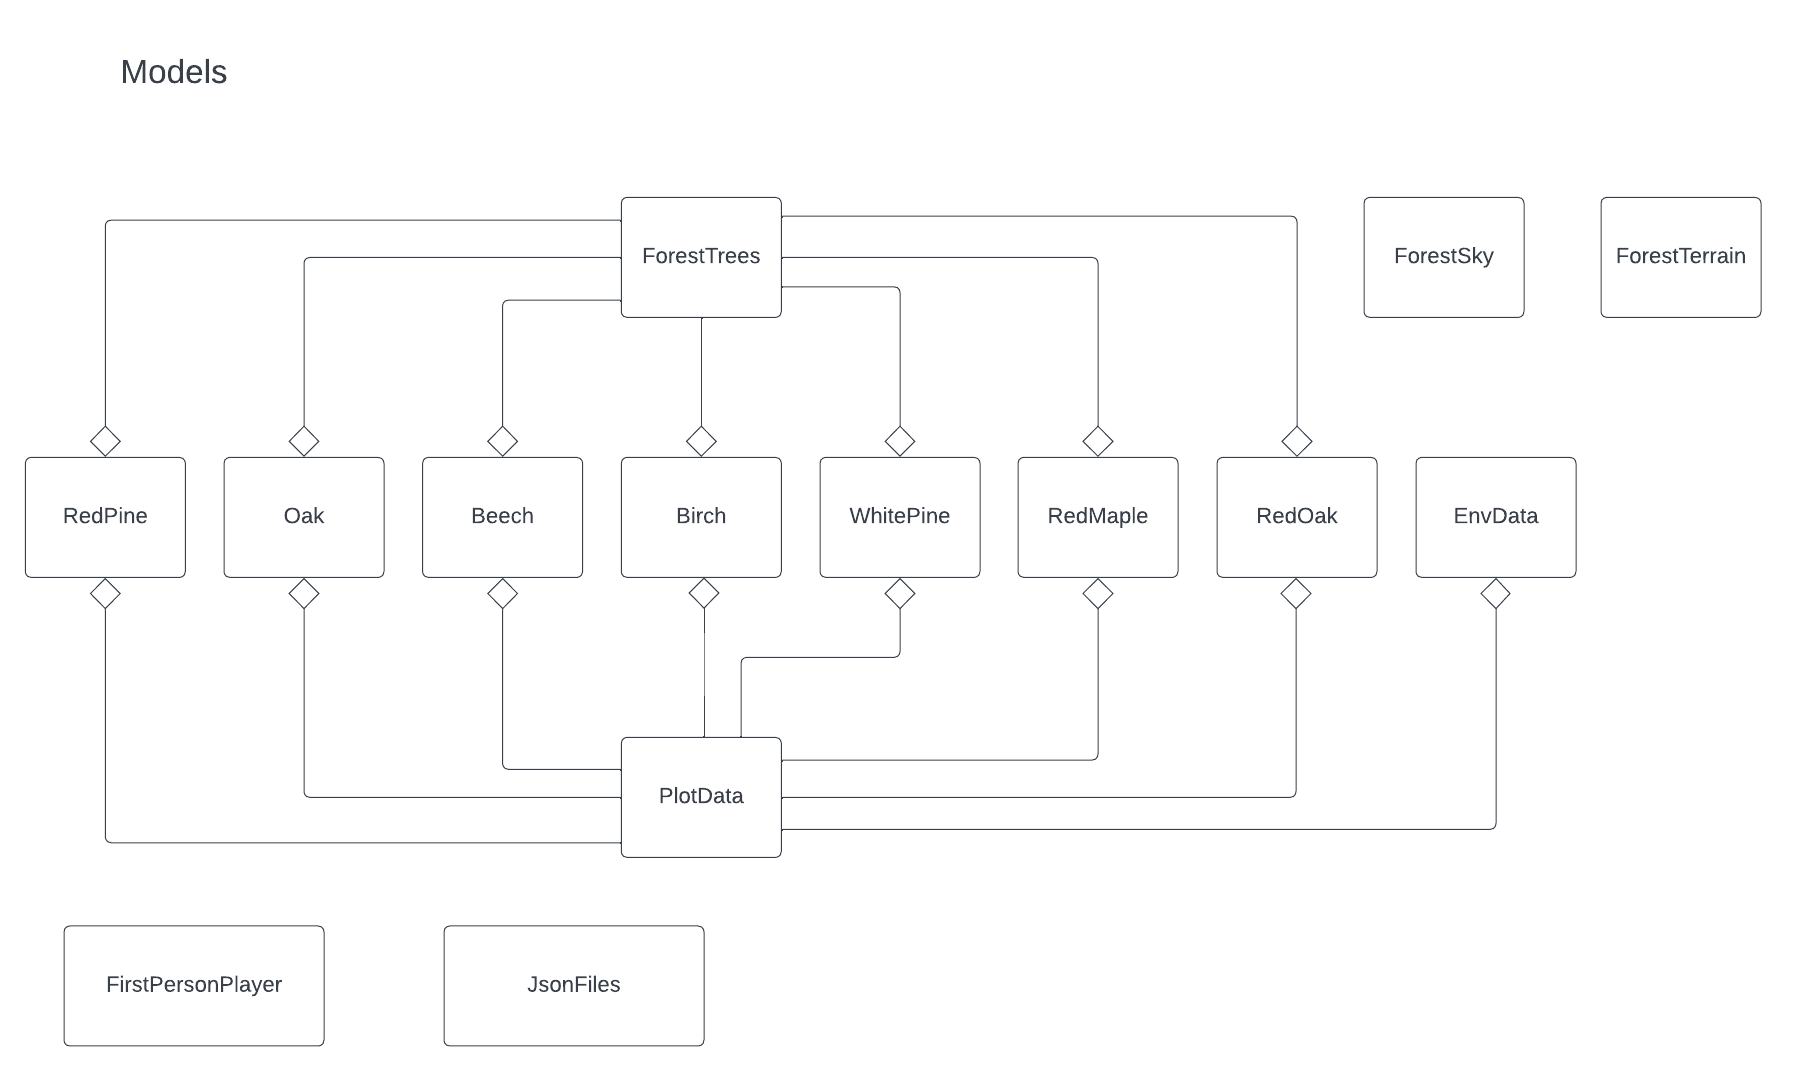
\includegraphics[scale=0.65]{Model-Modules.png}
\end{figure}

\newpage

\subsection{Relationship within Viewer Modules} \label{SecRBVM}
\begin{figure}[H]
\centering
\caption{Relationships within Viewer modules}
\label{FigRelaViewers}
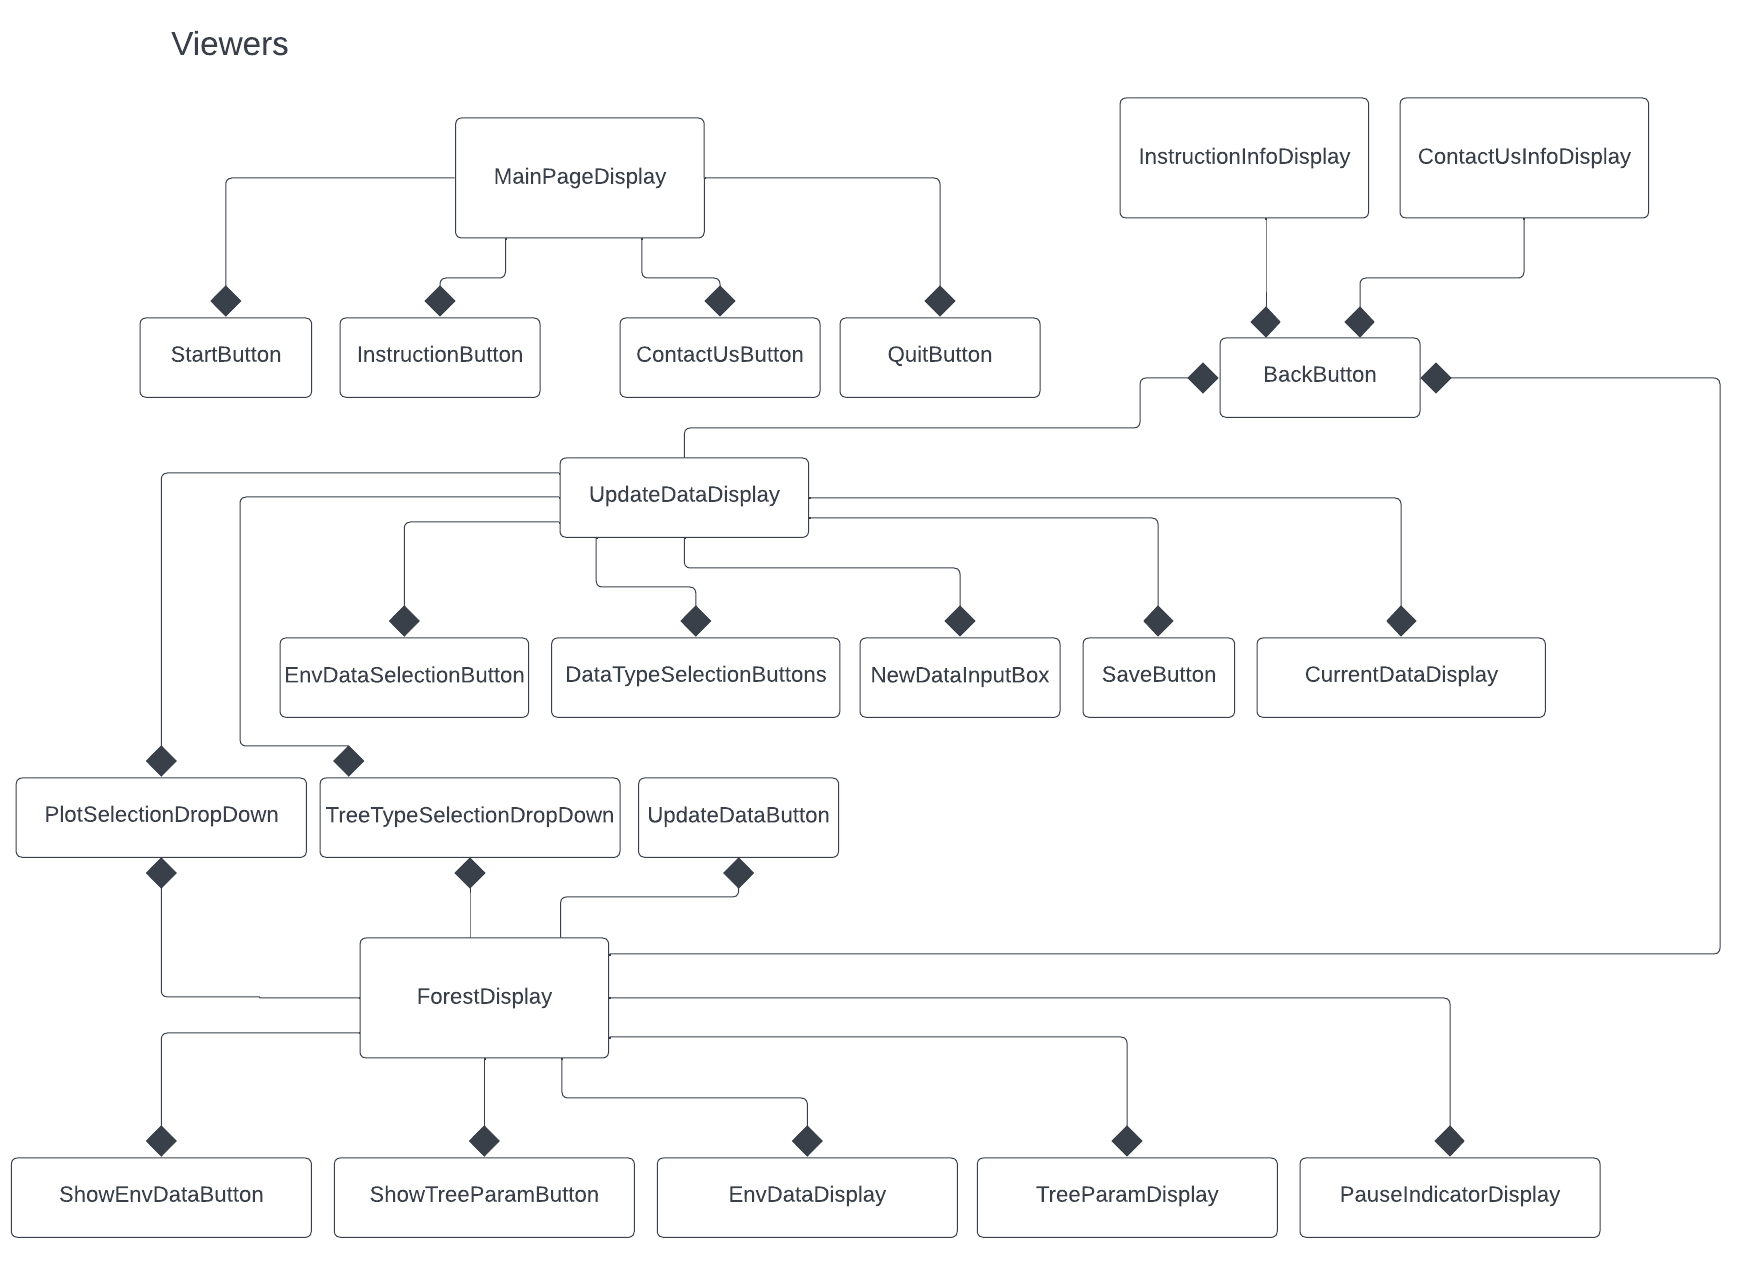
\includegraphics[scale=0.65]{Viewer-Modules.png}
\end{figure}

\newpage

\subsection{Relationship within Controller Modules} \label{SecRBCM}
\begin{figure}[H]
\centering
\caption{Relationships within Controller modules}
\label{FigRelaControllers}
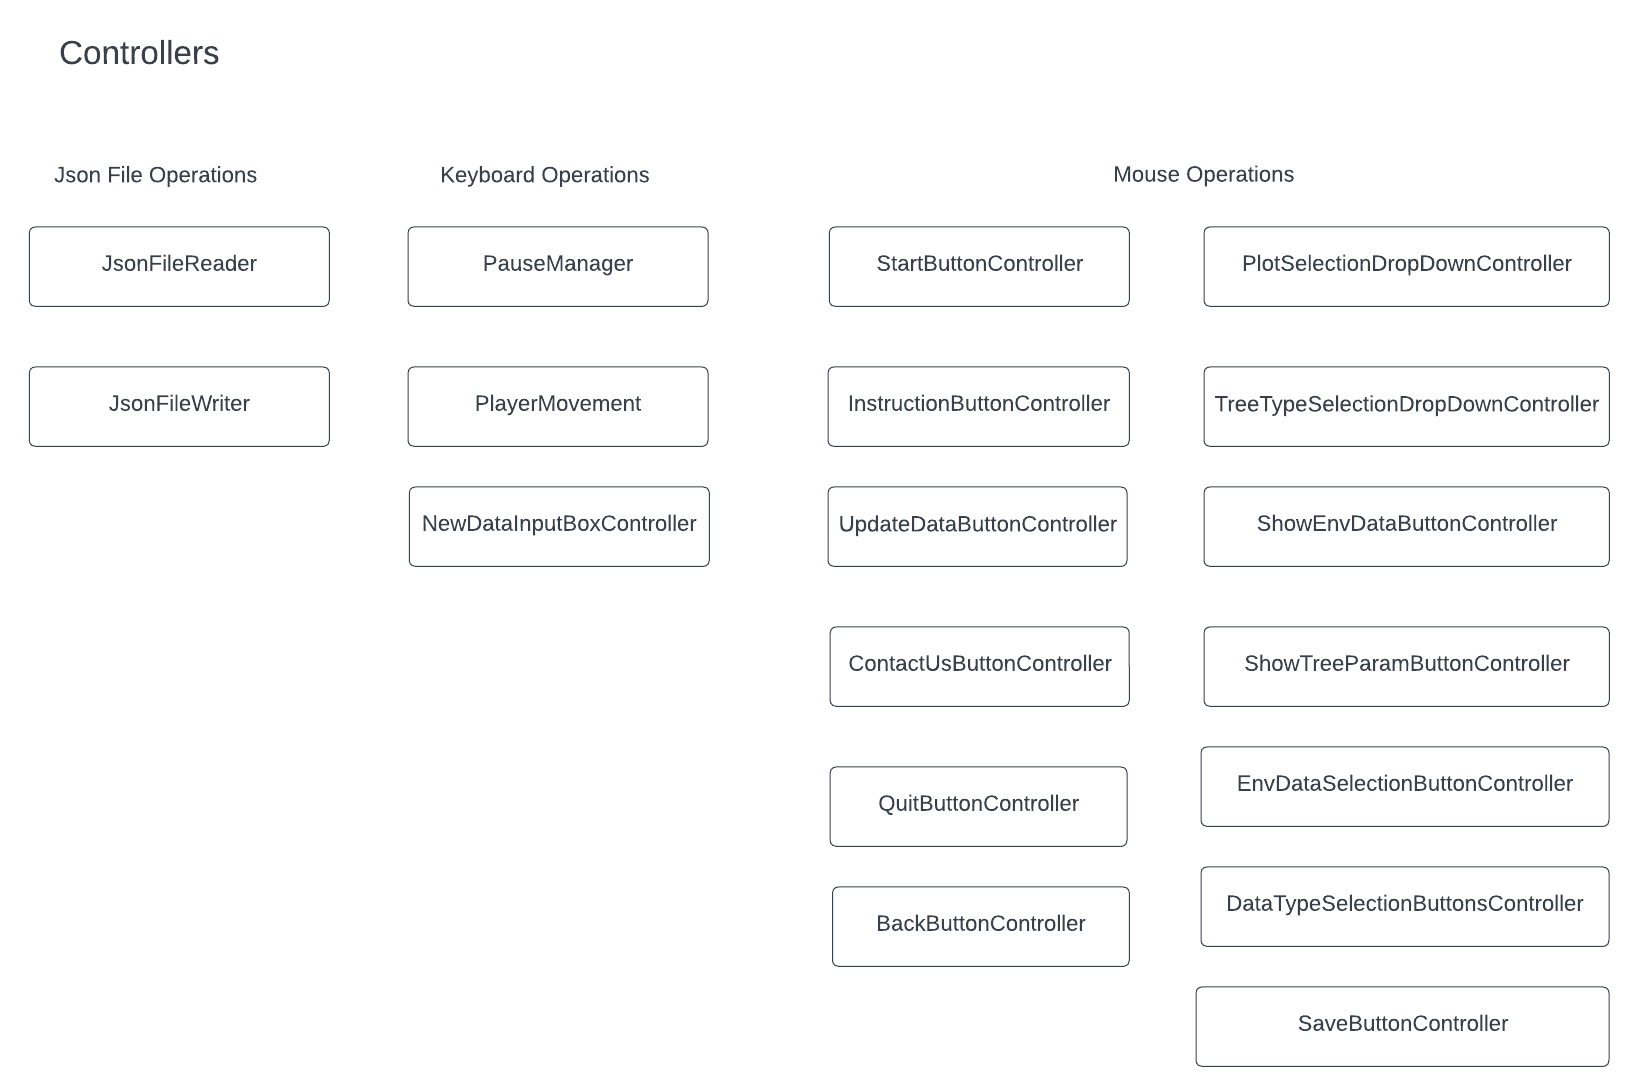
\includegraphics[scale=0.65]{Controller-Modules.png}
\end{figure}

\newpage

\subsection{Relationship between Model Modules, Viewer Modules, and Controller Modules} \label{SecRBMVC}
The following is a diagram to show the relationship between models, viewers, and controllers
of the MVC architecture.
\begin{figure}[H]
\centering
\caption{MVC Architecture}
\label{MVCArchitecture}
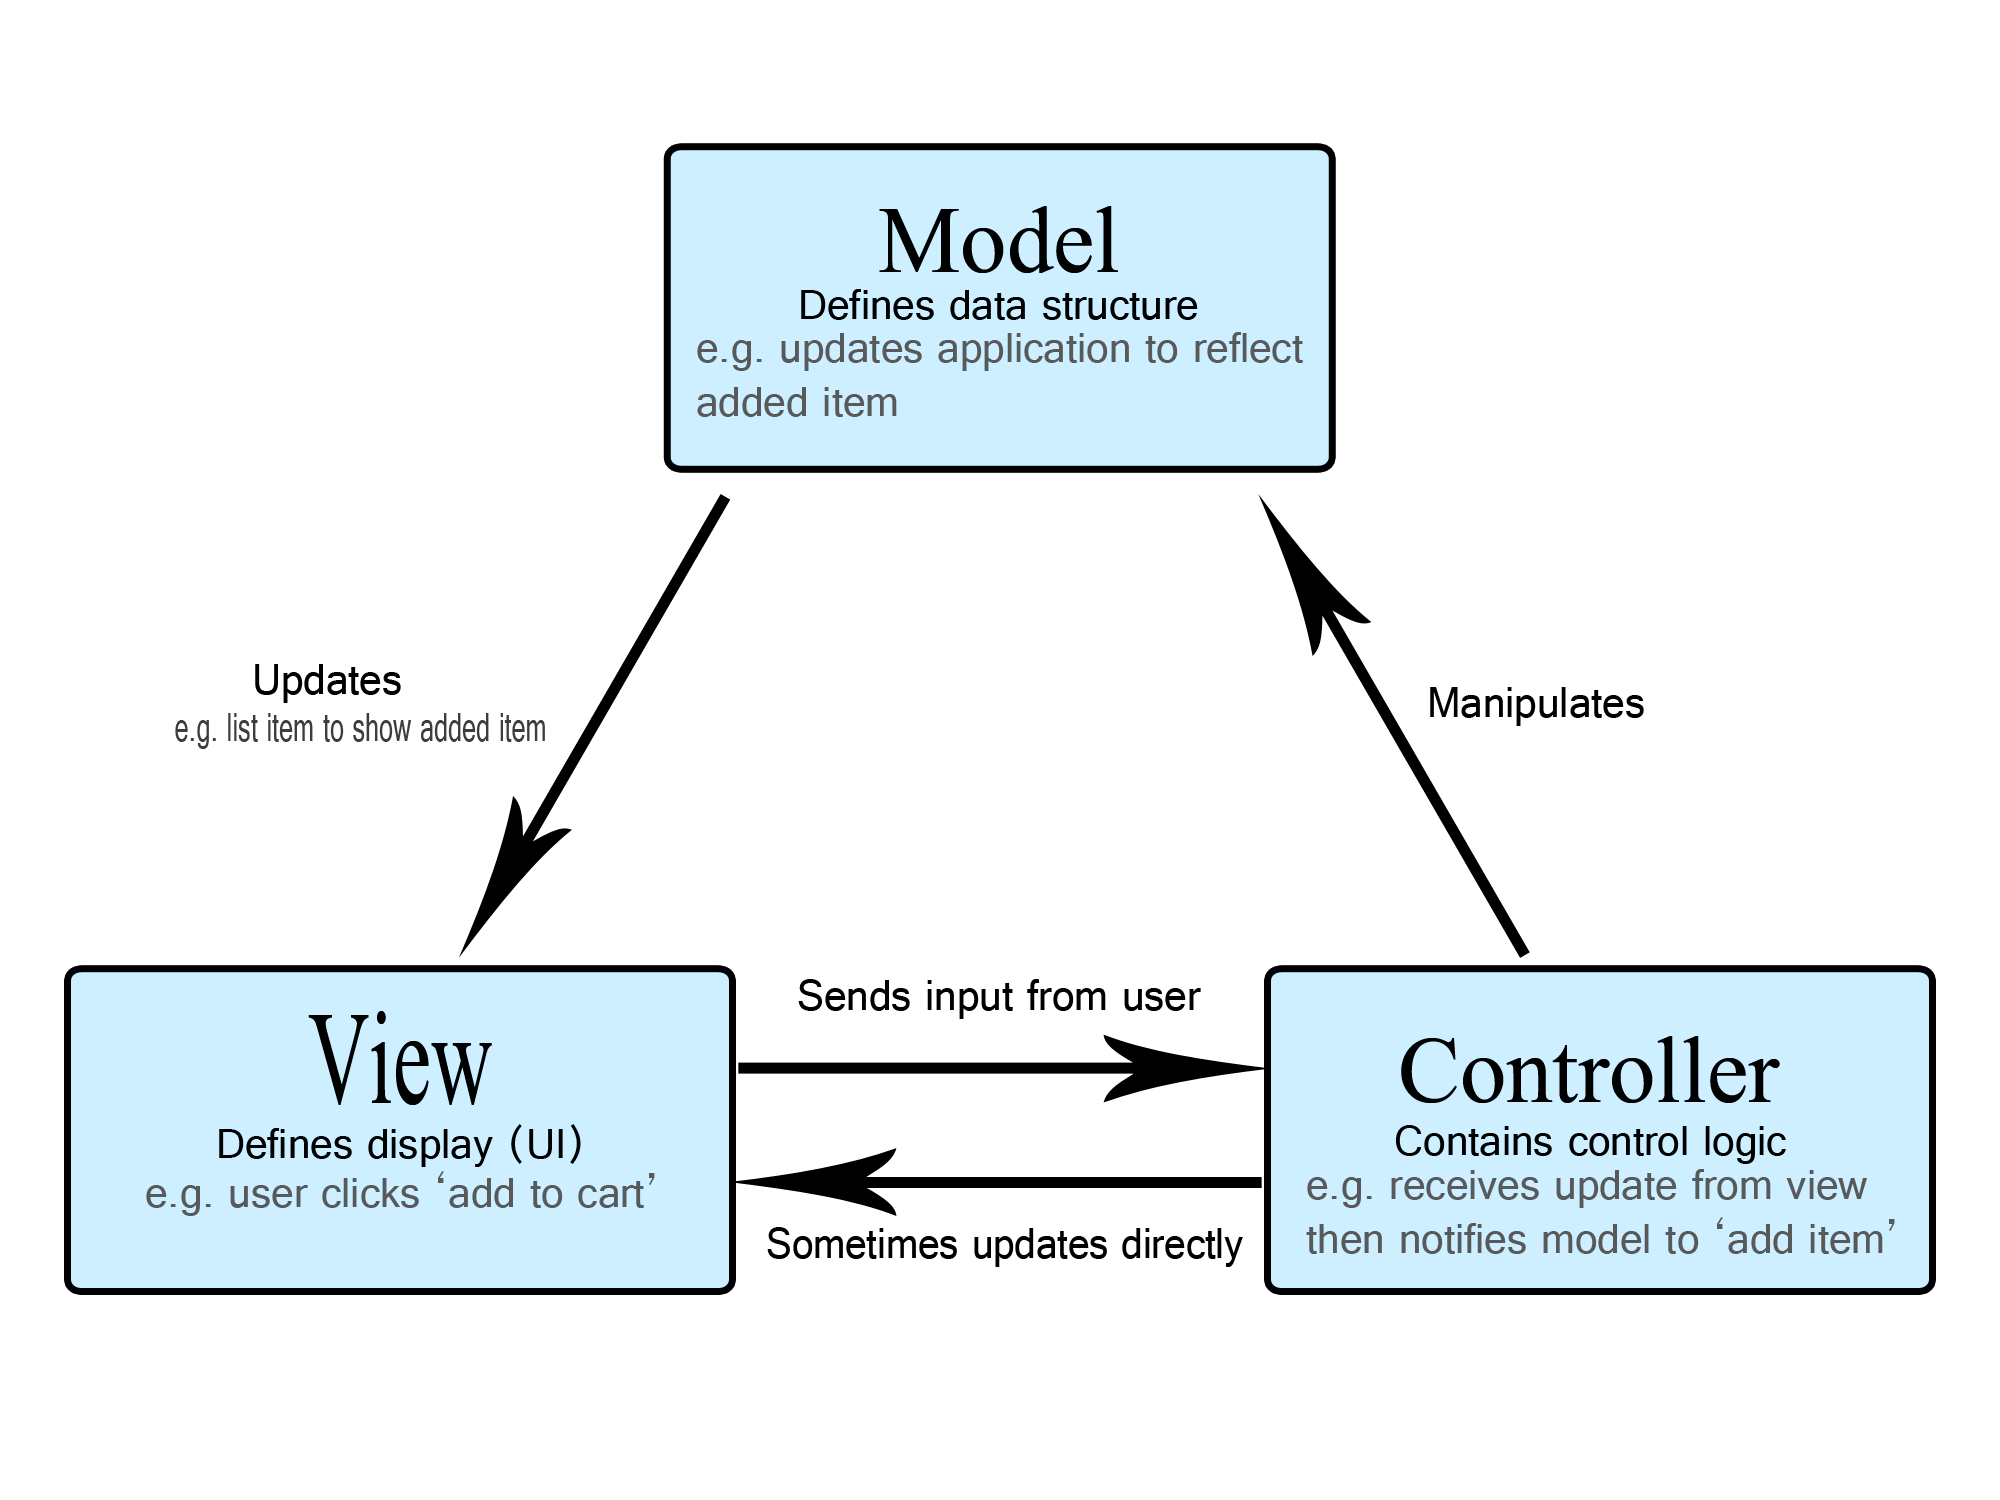
\includegraphics[scale=0.8]{MVC.png}
\end{figure}
\noindent Reference: Click \href{https://developer.mozilla.org/en-US/docs/Glossary/MVC}{here}.

\noindent Drawing graphs to represent relationships between Model modules, Viewer modules, and 
Controller modules is too complicated since we have many modules. Therefore, we chose to 
use words to describe relationships between between Model modules, Viewer modules, and 
Controller modules.

\newcommand{\vb}{\textbf{Updates }}
\subsubsection{Model Updates View}
\begin{itemize}
\item \mref{Model12} \vb \mref{Viwer21}
\item \mref{Model12} \vb \mref{Viwer22}
\item \mref{Model1} \vb \mref{Viwer18}
\item \mref{Model2} \vb \mref{Viwer18}
\item \mref{Model3} \vb \mref{Viwer18}
\end{itemize}

\renewcommand{\vb}{\textbf{Manipulates }}
\subsubsection{Controller Manipulates Model}
\begin{itemize}
\item \mref{Controller2} \vb \mref{Model14}
\item \mref{Controller4} \vb \mref{Model13}
\item \mref{Controller18} \vb \mref{Model12}
\end{itemize}

\renewcommand{\vb}{\textbf{Sends input from user to }}
\subsubsection{View Sends input from user to Controller}
\begin{itemize}
\item \mref{Viwer2} \vb \mref{Controller6}
\item \mref{Viwer3} \vb \mref{Controller7}
\item \mref{Viwer4} \vb \mref{Controller9}
\item \mref{Viwer8} \vb \mref{Controller11}
\item \mref{Viwer10} \vb \mref{Controller16}
\item \mref{Viwer11} \vb \mref{Controller17}
\item \mref{Viwer13} \vb \mref{Controller18}
\item \mref{Viwer15} \vb \mref{Controller12}
\item \mref{Viwer16} \vb \mref{Controller13}
\item \mref{Viwer17} \vb \mref{Controller8}
\item \mref{Viwer19} \vb \mref{Controller14}
\item \mref{Viwer20} \vb \mref{Controller15}
\end{itemize}

\renewcommand{\vb}{\textbf{Updates }}
\subsubsection{Controller Updates View}
\begin{itemize}
\item \mref{Controller3} \vb  \mref{Viwer23}
\item \mref{Controller6} \vb  \mref{Viwer18}
\item \mref{Controller7} \vb  \mref{Viwer6}
\item \mref{Controller9} \vb  \mref{Viwer7}
\item \mref{Controller14} \vb  \mref{Viwer21}
\item \mref{Controller15} \vb  \mref{Viwer22}
\item \mref{Controller16} \vb  \mref{Viwer11}
\item \mref{Controller17} \vb  \mref{Viwer11}
\end{itemize}
\newpage
\bibliographystyle {plainnat}
\bibliography{References}


\end{document}